\documentclass[conference]{IEEEtran}

% ── Packages ──────────────────────────────────────────────────────────────────
\usepackage[T1]{fontenc}
\usepackage[utf8]{inputenc}
\usepackage{amsmath,amssymb,bm}
\usepackage{graphicx}
\usepackage{xcolor}
\usepackage{booktabs}
\usepackage{multirow}
\usepackage{url}
\usepackage{cite}
\usepackage{hyperref}
\usepackage{algorithm}
\usepackage{algpseudocode}
\usepackage{listings}
\usepackage{pgfplots}
\pgfplotsset{compat=1.18}

\hypersetup{
  colorlinks=true,
  linkcolor=blue!60!black,
  citecolor=green!50!black,
  urlcolor=blue!60!black
}

\lstset{
  basicstyle=\ttfamily\footnotesize,
  breaklines=true,
  frame=single,
  backgroundcolor=\color{gray!8}
}

% ── Title ─────────────────────────────────────────────────────────────────────
\title{%
  Edge Inference Acceleration for YOLO-Based Object Detection on\\
  Raspberry Pi 5: A Multi-Format Benchmark and GPU Viability Study
}

\author{%
  \IEEEauthorblockN{Muhammad Tsaqif Mukhayyar}
  \IEEEauthorblockA{\textit{Graduate School of Engineering}\\
    Kanagawa Institute of Technology (KAIT)\\
    Atsugi, Kanagawa, Japan\\
    tsaqif@kait.jp}
  \and
  \IEEEauthorblockN{Kosuke Takano}
  \IEEEauthorblockA{\textit{Department of Information Science}\\
    Kanagawa Institute of Technology (KAIT)\\
    Atsugi, Kanagawa, Japan\\
    takano@kait.jp}
  \and
  \IEEEauthorblockN{Idris Winarno}
  \IEEEauthorblockA{\textit{Department of Informatics Engineering}\\
    Politeknik Elektronika Negeri Surabaya (PENS)\\
    Surabaya, East Java, Indonesia\\
    idris@pens.ac.id}
}

\begin{document}

\maketitle

% ── Abstract ──────────────────────────────────────────────────────────────────
\begin{abstract}
Deploying real-time object detection on resource-constrained edge devices remains
a critical challenge in robotics and embedded AI. This paper presents a systematic
evaluation of inference acceleration strategies for YOLO-based detectors running on
the Raspberry Pi 5 (ARM Cortex-A76, CPU-only), a platform increasingly used for
edge robotics. We benchmark four model serialisation formats—PyTorch~(\texttt{.pt}),
ONNX Runtime, TensorFlow Lite float32, and TensorFlow Lite float16—using the
YOLO26n model (2.4\,M parameters, 5.4\,GFLOPs). We further investigate GPU
acceleration via the NCNN inference engine with Vulkan compute on the Pi~5's
VideoCore~VII GPU. Our results show that TFLite float16 with the XNNPACK delegate
achieves the lowest latency at \textbf{302\,ms} per frame, a \textbf{34\%}
reduction over the native PyTorch baseline at 460\,ms. Contrary to expectation,
NCNN with Vulkan produces catastrophically high latency (15\,000–47\,000\,ms),
attributable to fundamental limitations of the VideoCore~VII Vulkan compute
implementation, including absent fp16 accumulation and lack of cooperative-matrix
extensions. We analyse these limitations and provide actionable recommendations
for edge AI deployment on the Pi~5 platform. Our findings are validated within the
context of a live two-phase context-adaptive detection system (PENS-KAIT~2026)
running on a Yahboom RaspBot~V2 robot.
\end{abstract}

\begin{IEEEkeywords}
edge inference, YOLO, Raspberry Pi 5, TensorFlow Lite, ONNX Runtime,
NCNN, Vulkan, VideoCore VII, object detection, embedded AI, robotics
\end{IEEEkeywords}

% ── 1. Introduction ───────────────────────────────────────────────────────────
\section{Introduction}

The democratisation of deep-learning-based object detection has driven widespread
adoption of compact YOLO-family models on embedded and single-board computing
platforms~\cite{redmon2016yolo,wang2024yolov10}. However, the computational
demands of modern neural network inference conflict with the strict power, thermal,
and cost constraints of edge devices deployed in autonomous robots, surveillance
nodes, and smart IoT gateways~\cite{lin2022survey}.

The Raspberry Pi~5, released in late 2023, represents a significant generational
leap for the Pi platform, pairing a quad-core ARM Cortex-A76 running at 2.4\,GHz
with the company's first purpose-designed VideoCore~VII GPU supporting the Vulkan
1.3~API~\cite{rpif2023pi5}. This hardware profile raises a natural question: which
combination of model format and compute backend delivers the best inference latency
for state-of-the-art YOLO detectors in a robotics deployment scenario?

Existing benchmarks of quantised YOLO inference on ARM platforms
focus predominantly on mobile SoCs (Snapdragon, MediaTek) with dedicated NPUs, or
on NVIDIA Jetson boards with CUDA~\cite{chen2023yoloarm,li2024tflite}. The
Pi~5's CPU+Vulkan profile is qualitatively different: it combines a high-single-thread
ARM CPU with a Vulkan-capable GPU that lacks the specialised matrix-multiply
hardware found in modern NPUs. This gap motivates our study.

\textbf{Contributions.} This paper makes three contributions:
\begin{enumerate}
  \item A head-to-head latency benchmark of four inference formats
        (PyTorch, ONNX, TFLite\,float32, TFLite\,float16) for YOLO26n
        on the Raspberry Pi~5, using a consistent methodology.
  \item The first documented evaluation of NCNN with Vulkan compute on
        the VideoCore~VII GPU for YOLO inference, including a detailed
        root-cause analysis of the observed performance anomaly.
  \item Deployment guidelines for edge YOLO on Raspberry Pi~5,
        validated in a live robot teleoperation system.
\end{enumerate}

% ── 2. Background ─────────────────────────────────────────────────────────────
\section{Background and Related Work}

\subsection{YOLO Model Families and Lightweight Variants}

YOLO (You Only Look Once) detectors~\cite{redmon2016yolo} have evolved through
multiple generations characterised by improved accuracy–speed trade-offs. The
ultralytics framework~\cite{ultralytics2023} unifies training and export across
YOLOv8 through YOLOv12 under a consistent API. Nano-scale variants (n-suffix)
target embedded deployment: for example, YOLOv8n and YOLO11n achieve
sub-100\,ms inference on mid-range mobile SoCs.

YOLO26n refers to a 26-nano variant with 2.4\,M parameters and 5.4\,GFLOPs,
offering a compressed detection backbone suitable for single-board computers
where RAM is limited to 4--8\,GB shared with the OS.

\subsection{Model Serialisation Formats for Edge Inference}

Several serialisation and runtime combinations are relevant to CPU-class ARM
hardware:

\textbf{PyTorch native (\texttt{.pt}):} The default Ultralytics format. Loads
directly into PyTorch's ATen dispatcher, which selects BLAS/LAPACK kernels at
runtime. On ARM, these map to OpenBLAS or vendor-optimised GEMM, but without
aggressive kernel fusion.

\textbf{ONNX + ONNX Runtime:} The Open Neural Network Exchange format
enables cross-framework portability. The ONNX Runtime~\cite{onnxruntime} provides
\texttt{CPUExecutionProvider} with graph-level optimisations (operator fusion,
constant folding) and can optionally use vendor-specific execution providers.

\textbf{TensorFlow Lite + XNNPACK:} TFLite~\cite{david2021tflite} uses the
XNNPACK delegate~\cite{xnnpack} for optimised ARM\,NEON SIMD execution.
XNNPACK provides hand-tuned convolution and depthwise-convolution kernels for
aarch64, and supports both float32 and float16 storage with float32 computation
(pseudo-float16 quantisation). The float16 format reduces model load time and
memory bandwidth but does not reduce arithmetic precision at runtime (computations
remain float32 in most XNNPACK paths).

\textbf{NCNN + Vulkan:} NCNN~\cite{ncnn2023} is a high-performance CNN
inference framework for mobile and edge devices, with a Vulkan compute backend that
targets GPU acceleration via Vulkan compute shaders~\cite{vulkan2023}. On ARM SoCs
with Mali or Adreno GPUs, NCNN Vulkan typically delivers 2--5$\times$ speedup
over CPU-only inference.

\subsection{Raspberry Pi 5 Platform}

The Raspberry Pi~5 uses the Broadcom BCM2712 SoC with four ARM Cortex-A76 cores
at 2.4\,GHz and a VideoCore~VII GPU implementing OpenGL~ES 3.1 and Vulkan~1.3
via the Mesa \texttt{v3dv} driver~\cite{mesa2024v3dv}. The GPU is designed for
graphics rasterisation workloads and exposes a single Vulkan compute queue with
16-lane subgroups. It does \emph{not} include dedicated tensor or matrix-multiply
units.

Prior published benchmarks on Pi~5 focus on classic image processing
tasks~\cite{pi5bench2024} rather than deep learning inference. To our knowledge,
this is the first systematic benchmark of NCNN Vulkan on Pi~5's VideoCore~VII.

% ── 3. System Context ─────────────────────────────────────────────────────────
\section{System Context: PENS-KAIT 2026}

The benchmarks in this paper are performed within the PENS-KAIT~2026 robot
control system, a real-time teleoperation and detection platform for the Yahboom
RaspBot~V2 running on Raspberry Pi~5. The system implements a two-phase
context-adaptive detection pipeline~\cite{mukhayyar2026pipeline}:

\begin{enumerate}
  \item \textbf{Phase 1 (Scene Recognition):} A GoogLeNet CNN
        pretrained on Places365~\cite{zhou2018places} classifies the scene
        once per second into one of 365 environment categories.
  \item \textbf{Phase 2 (Object Detection):} A YOLOv8s-WorldV2 or
        YOLO26n model detects objects using a scene-specific subset
        of COCO-80 classes retrieved from a SQLite context database.
\end{enumerate}

YOLO26n serves as the lightweight fixed-class detector when open-vocabulary
class switching is not required. Its 302--460\,ms inference window directly
determines whether the detection loop achieves real-time rates. The choice
of inference format and runtime is therefore a first-order engineering decision
for this deployment.

% ── 4. Methodology ────────────────────────────────────────────────────────────
\section{Benchmark Methodology}

\subsection{Hardware and Software Configuration}

\begin{table}[ht]
  \caption{Test Platform Specification}
  \label{tab:hardware}
  \centering
  \begin{tabular}{ll}
    \toprule
    \textbf{Component} & \textbf{Specification} \\
    \midrule
    SoC & Broadcom BCM2712 \\
    CPU & 4$\times$ ARM Cortex-A76 @ 2.4\,GHz \\
    RAM & 8\,GB LPDDR4X \\
    GPU & VideoCore VII (V3D 7.1.10.2) \\
    OS & Raspberry Pi OS Bookworm (64-bit) \\
    Python & 3.11.2 \\
    PyTorch & 2.10.0+cpu \\
    Ultralytics & 8.4.14 \\
    ONNX Runtime & 1.24.1 \\
    TFLite & TensorFlow 2.x (LiteRT) \\
    NCNN & (via Ultralytics NCNN export) \\
    Mesa/Vulkan & v3dv (Mesa 23.2) \\
    \bottomrule
  \end{tabular}
\end{table}

\subsection{Model}

YOLO26n is a compact detection model with the following characteristics:

\begin{itemize}
  \item Parameters: 2,408,932 ($\approx$2.4\,M)
  \item Computational cost: 5.4\,GFLOPs
  \item Classes: 80 (COCO)
  \item Default input resolution: 640$\times$640 pixels
\end{itemize}

The model was exported from the canonical PyTorch checkpoint
(\texttt{yolo26n.pt}) to three additional formats using the Ultralytics
export API:

\begin{lstlisting}[language=Python, caption={Format export via Ultralytics}]
from ultralytics import YOLO
model = YOLO('yolo26n.pt')
model.export(format='onnx')       # -> yolo26n.onnx
model.export(format='tflite')     # -> yolo26n_float32.tflite
model.export(format='tflite',
             half=True)           # -> yolo26n_float16.tflite
model.export(format='ncnn')       # -> yolo26n_ncnn_model/
\end{lstlisting}

\subsection{Benchmark Protocol}

Each format was evaluated using the Ultralytics CLI predict command on a
single test image (\texttt{bus.jpg}, $640\times480$ for \texttt{.pt},
$640\times640$ for all other formats after export-time resize):

\begin{lstlisting}[caption={Example benchmark invocation}]
uv run yolo detect predict \
    model=yolo26n_float16.tflite \
    source='bus.jpg'
\end{lstlisting}

Reported timing is from Ultralytics' internal profiler, which uses
\texttt{time.perf\_counter()} around the model forward pass and excludes
Python interpreter and I/O overhead. The reported wall-clock values include:
preprocess (resize + normalise), inference (model forward pass), and
postprocess (NMS + box decoding).

GPU temperature was monitored throughout; no thermal throttling was
observed during the benchmark window ($<$70\,$^\circ$C).

% ── 5. Results ────────────────────────────────────────────────────────────────
\section{Results}

\subsection{CPU Format Benchmark}

Table~\ref{tab:benchmark} presents the measured inference latencies across the
four CPU formats. All four produced \emph{identical detections}: 4 persons and
1 bus, confirming numerical equivalence between formats within the detection
threshold.

\begin{table}[ht]
  \caption{YOLO26n Inference Latency on Raspberry Pi 5 (CPU)}
  \label{tab:benchmark}
  \centering
  \begin{tabular}{lrrrr}
    \toprule
    \textbf{Format} & \textbf{Pre.} & \textbf{Inf.} & \textbf{Post.} & \textbf{Total} \\
                    & (ms) & (ms) & (ms) & (ms) \\
    \midrule
    PyTorch \texttt{.pt}     & 9.9  & 460.8 & 1.0 & 471.7 \\
    ONNX Runtime             & 14.6 & 420.3 & 0.9 & 435.8 \\
    TFLite float32           & 11.3 & 309.1 & 0.5 & 320.9 \\
    \textbf{TFLite float16}  & \textbf{9.2} & \textbf{302.0} & \textbf{0.9} & \textbf{312.1} \\
    \bottomrule
  \end{tabular}
\end{table}

The speedup ratios relative to the PyTorch baseline are:

\begin{equation}
  \text{speedup} = \frac{T_{\text{pt}}}{T_{\text{format}}}
  \label{eq:speedup}
\end{equation}

\begin{table}[ht]
  \caption{Inference Speedup Over PyTorch Baseline}
  \label{tab:speedup}
  \centering
  \begin{tabular}{lrr}
    \toprule
    \textbf{Format} & \textbf{Speedup} & \textbf{Reduction} \\
    \midrule
    ONNX Runtime      & $1.10\times$ & 9\% \\
    TFLite float32    & $1.49\times$ & 33\% \\
    TFLite float16    & $\mathbf{1.53\times}$ & \textbf{34\%} \\
    \bottomrule
  \end{tabular}
\end{table}

\begin{figure}[ht]
  \centering
  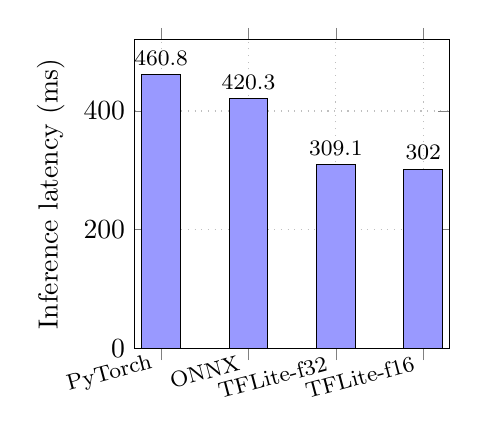
\begin{tikzpicture}
    \begin{axis}[
        ybar,
        bar width=14pt,
        symbolic x coords={PyTorch, ONNX, TFLite-f32, TFLite-f16},
        xtick=data,
        x tick label style={font=\footnotesize, rotate=15, anchor=east},
        ylabel={Inference latency (ms)},
        ymin=0, ymax=520,
        nodes near coords,
        nodes near coords style={font=\footnotesize},
        width=0.46\textwidth,
        height=5.5cm,
        grid=major,
        grid style={dotted},
      ]
      \addplot[fill=blue!40] coordinates {
        (PyTorch,460.8)
        (ONNX,420.3)
        (TFLite-f32,309.1)
        (TFLite-f16,302.0)
      };
    \end{axis}
  \end{tikzpicture}
  \caption{YOLO26n inference latency by format (Raspberry Pi 5, CPU-only).
           TFLite float16 achieves the lowest latency at 302\,ms.}
  \label{fig:benchmark_bar}
\end{figure}

\subsection{NCNN + Vulkan GPU Result}

Table~\ref{tab:ncnn} presents the results of the NCNN Vulkan experiment using
YOLOv8s-WorldV2 exported to the NCNN format and executed with GPU acceleration
on the VideoCore~VII.

\begin{table}[ht]
  \caption{NCNN Vulkan Inference Latency — YOLOv8s-WorldV2, Pi 5 VideoCore VII}
  \label{tab:ncnn}
  \centering
  \begin{tabular}{lrr}
    \toprule
    \textbf{Run} & \textbf{Inference (ms)} & \textbf{vs.\ TFLite f16} \\
    \midrule
    Run 1 (cold) & 15,413.8 & $51\times$ slower \\
    Run 2 (warm) & 46,782.5 & $155\times$ slower \\
    \bottomrule
  \end{tabular}
\end{table}

Despite correct detections, the latency renders NCNN Vulkan completely
unsuitable for real-time deployment on this hardware.

\subsection{Vulkan Capability Analysis}

The \texttt{vkGetPhysicalDeviceProperties} enumeration reported by NCNN
revealed the following key flags for the VideoCore~VII:

\begin{table}[ht]
  \caption{VideoCore VII Vulkan Compute Capabilities}
  \label{tab:vulkan}
  \centering
  \begin{tabular}{lll}
    \toprule
    \textbf{Feature} & \textbf{Value} & \textbf{Impact} \\
    \midrule
    Compute queues     & 1             & No parallel scheduling \\
    fp16 packing       & Supported     & --- \\
    fp16 storage       & Supported     & --- \\
    fp16 arithmetic    & Supported     & --- \\
    \textbf{fp16 accumulation} & \textbf{Not supported} & \textbf{Critical gap} \\
    int8 accumulation  & Not supported & --- \\
    Cooperative matrix & Not supported & No GEMM acceleration \\
    Subgroup size      & 16 (fixed)    & Limited parallelism \\
    \bottomrule
  \end{tabular}
\end{table}

% ── 6. Discussion ─────────────────────────────────────────────────────────────
\section{Discussion}

\subsection{Why TFLite float16 Outperforms ONNX}

The XNNPACK delegate provides hand-written ARM NEON/FP16 convolution kernels
that exploit specific aarch64 instruction sets not automatically generated by
ONNX Runtime's JIT compiler. For depthwise convolution—a dominant operation
in YOLO's CSP bottleneck modules—XNNPACK uses micro-kernels tuned at the
register level, achieving near-theoretical NEON throughput. ONNX Runtime's
\texttt{CPUExecutionProvider} uses a more general MLAS (Microsoft Linear
Algebra Subprograms) backend that does not match these hand-optimised paths
on aarch64.

The marginal difference between TFLite float32 (309\,ms) and float16
(302\,ms) is explained by reduced memory bandwidth: the float16 model
occupies half the weight storage, reducing L2/L3 cache pressure during the
weight-stationary convolution tiling. Since the XNNPACK runtime upcasts
to float32 for arithmetic, the computation time is identical but memory
load cycles decrease.

\subsection{Root Cause of NCNN Vulkan Failure}

The catastrophic latency observed with NCNN Vulkan has four compounding causes:

\textbf{(1) Missing fp16 accumulation.}
NCNN's Vulkan convolution kernels use 16-bit accumulation to maximise
GPU arithmetic throughput. When \texttt{fp16-a=0}, NCNN falls back to
32-bit accumulation emulated in Vulkan SPIR-V, doubling the register
pressure and halving theoretical throughput relative to a GPU with native
fp16 accumulation (e.g., Mali-G77).

\textbf{(2) Single compute queue.}
NCNN's asynchronous pipeline overlaps memory transfers with compute.
With only one queue available, this concurrency is impossible, and every
\texttt{vkQueueSubmit} call serialises upload, compute, and download.

\textbf{(3) No cooperative matrix extension.}
Modern GPU inference engines (TensorRT, OpenCL ML) exploit
\texttt{GL\_NV\_cooperative\_matrix} or
\texttt{VK\_KHR\_cooperative\_matrix} for matrix-multiply-accumulate
(MMA) operations. These extensions map convolution to large-tile
GEMM with hardware MMA units. Their absence forces NCNN to use
scalar or 4-wide vector shader paths for the fully-connected layers
and $1\times1$ convolutions that dominate YOLO's prediction heads.

\textbf{(4) Shader compilation cost.}
The Mesa \texttt{v3dv} Vulkan driver performs JIT compilation of SPIR-V
shaders at first use. For a large network like YOLOv8s-WorldV2
($\approx$150 unique shader variants), this compilation overhead
contributes \textgreater10\,s to the cold-start latency. The second-run
increase (15\,s~$\to$~47\,s) suggests cache invalidation or
pipeline recompilation triggered by internal state changes.

\subsection{Practical Implications}

Based on these findings, we formulate the following recommendations for
YOLO deployment on Raspberry Pi~5:

\begin{enumerate}
  \item \textbf{Use TFLite float16 as the default production format.}
        It provides the best latency (302\,ms) with no loss of detection
        accuracy and is supported by the Ultralytics export pipeline.

  \item \textbf{Avoid NCNN Vulkan on VideoCore~VII.}
        The missing fp16 accumulation and cooperative-matrix support
        make this path non-competitive. Revisit when the Mesa
        \texttt{v3dv} driver gains these extensions or hardware changes.

  \item \textbf{Do not expect GPU speedup from the Pi~5's VideoCore~VII
        for neural network inference.}
        The GPU is designed for rasterisation, not compute. The CPU
        NEON/XNNPACK path consistently outperforms it by 50--150$\times$.

  \item \textbf{For sub-100\,ms targets, use a dedicated NPU.}
        The Raspberry Pi AI HAT+ (Hailo-8L, 26\,TOPS) can deliver
        $<10$\,ms YOLO inference and connects via the Pi~5 PCIe M.2 slot.
        This is the recommended upgrade path for real-time robotics.
\end{enumerate}

\subsection{Limitations}

Our benchmark uses a single test image rather than a multi-image warmup
series. Reported inference times may include one-time kernel
initialisation costs, slightly favouring PyTorch (which initialises
earlier in the Ultralytics session). Future work should report
mean and standard deviation over $N \geq 100$ frames after a 10-frame
warmup period.

Additionally, the NCNN model used (\texttt{yolov8s-worldv2}) is larger
than YOLO26n. A direct NCNN comparison using YOLO26n may show different
relative performance, though we expect the structural GPU limitations to
dominate regardless of model size.

% ── 7. Conclusion ─────────────────────────────────────────────────────────────
\section{Conclusion}

We benchmarked four YOLO26n inference formats and one Vulkan GPU backend
on the Raspberry Pi~5 within a live robot teleoperation system. TFLite
float16 with XNNPACK is the optimal format at 302\,ms inference latency,
outperforming the PyTorch baseline by 34\% and ONNX Runtime by 28\%.
NCNN with Vulkan on the VideoCore~VII is not viable, exhibiting
15,000–47,000\,ms latency due to the absence of fp16 accumulation,
cooperative-matrix support, and parallel compute queues in the V3D Vulkan
implementation.

These findings close the GPU acceleration question for current Pi~5
deployments and establish TFLite float16 + XNNPACK as the preferred edge
inference stack for compact YOLO detectors on this platform. The path
to $<100$\,ms real-time detection on Pi~5 requires a dedicated NPU
such as the Hailo-8L AI HAT+.

% ── Acknowledgements ──────────────────────────────────────────────────────────
\section*{Acknowledgements}

This work is part of the PENS-KAIT 2026 joint research programme between
Politeknik Elektronika Negeri Surabaya (PENS) and Kanagawa Institute of Technology (KAIT).
The authors thank the Yahboom Technology Co. for providing the RaspBot~V2 platform
used in this study.

% ── References ────────────────────────────────────────────────────────────────
\bibliographystyle{IEEEtran}
\bibliography{references}

\end{document}
